%! suppress = LineBreak
%! suppress = Unicode
%! suppress = MissingLabel
%! suppress = MissingImport
%! suppress = FileNotFound
\documentclass[../main.tex]{subfiles}

\begin{document}
    \begin{figure}[H]
        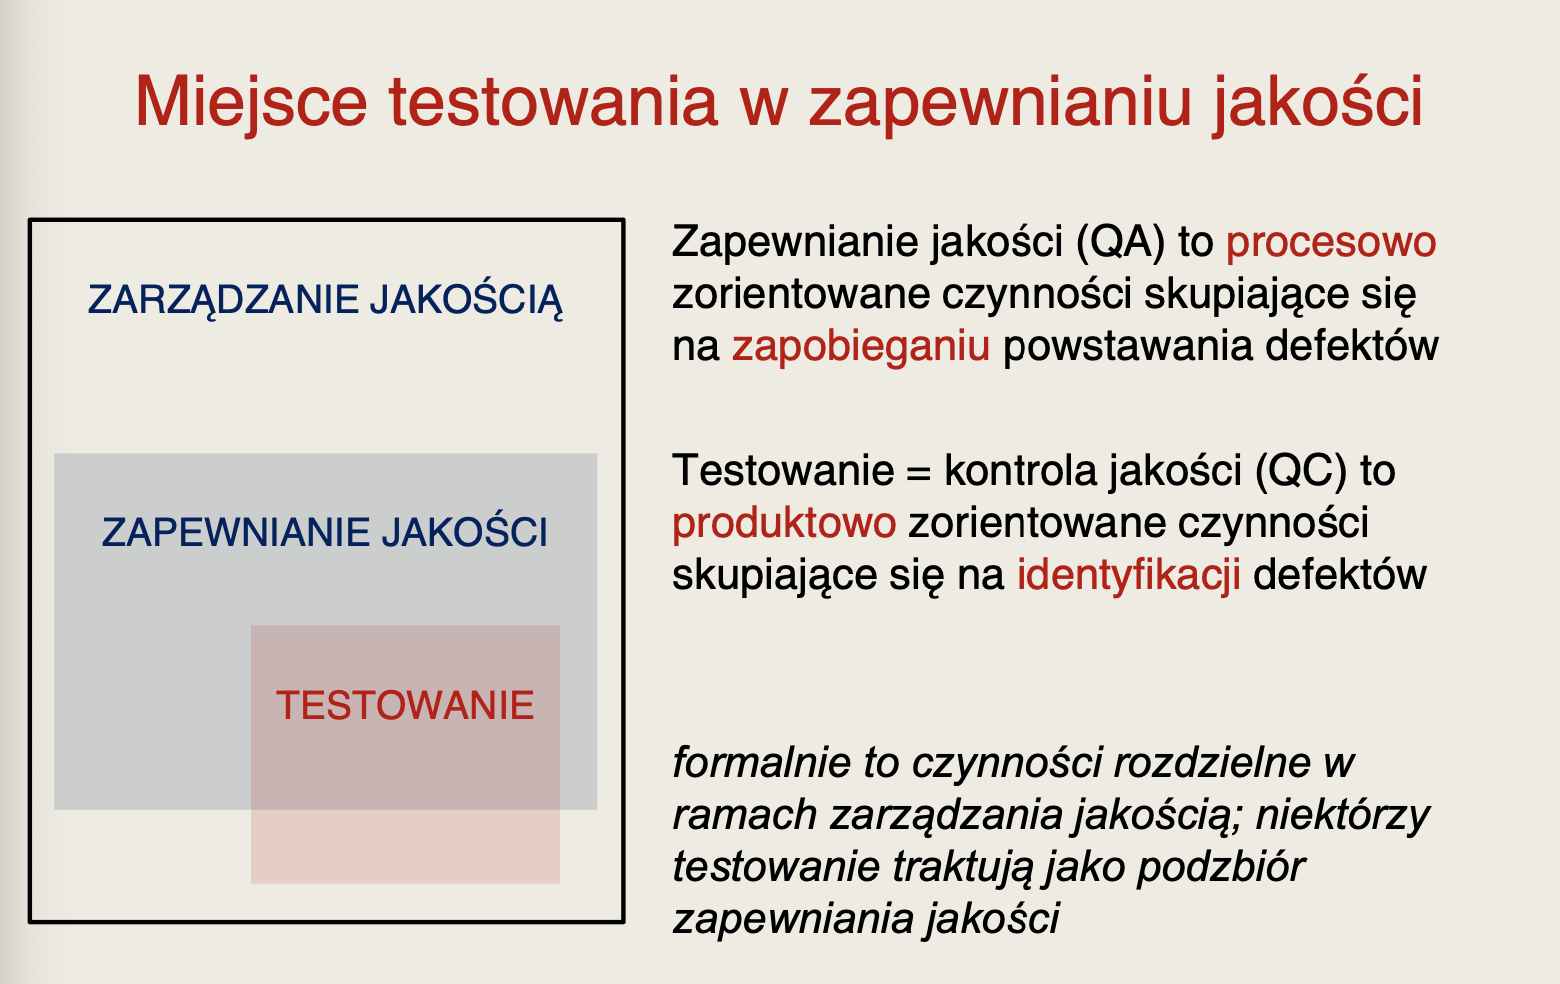
\includegraphics[width=\linewidth]{jakosc.png}
    \end{figure}

    \begin{table}[H]
        \begin{center}
            \begin{tabular}{| p{3cm} || p{6cm} | p{6cm} |}
                \hline
                & \textbf{Zapewnianie jakości (QA)} & \textbf{Testowanie (QC)}    \\
                \hline
                \hline
                \textbf{Cel} & Ulepszyć proces produkcji i testowania oprogramowania,
                aby defekty się nie pojawiały & Identyfikacja defektów po wyprodukowaniu produktu,
                a przed wydaniem do klienta \\
                \hline
                \textbf{Jak?} & Wdrożenie systemu zarządzania jakością; okresowe audyty &
                Znajdowanie i eliminowanie problemów z jakością aby wymagania klienta były spełnione \\
                \hline
                \textbf{Co?} & Zapobieganie problemom przez planowe i systematyczne działania
                & Wykorzystanie technik testowania do identyfikacji defektów \\
                \hline
                \textbf{Odpowiedzialność} & Wszyscy są odpowiedzialni         & Zwykle zespół testerski     \\
                \hline
                \textbf{Przykład}         & Weryfikacja                       & Walidacja, testowanie       \\
                \hline
                \textbf{Techniki}         & Statistical Process Control       & Statistical Quality Control \\
                \hline
                \textbf{Jako narzędzie}   & QA to narzędzia zarządcze         & QC to narzędzie korekcyjne  \\
                \hline
            \end{tabular}
        \end{center}
    \end{table}

    \begin{table}[H]
        \begin{center}
            \begin{tabular}{p{8cm} p{8cm}}
                \multicolumn{2}{c}{\textbf{Przykłady aktywności QA.}} \\
                \begin{itemize}
                    \item \textbf{definiowanie i implementacja procesów}
                    \begin{itemize}
                        \item metodyka wytwarzania oprogramowania
                        \item zarządzanieprojektami
                        \item zarządzanie konfiguracją
                        \item zarządzanie wymaganiami
                        \item metody pomiaru oprogramowania, szacowanie – projektowanie oprogramowania
                        \item proces testowy
                    \end{itemize}
                \end{itemize}
                &
                \begin{itemize}
                    \item \textbf{identyfikacja słabych punktów} w procesach i ciągła poprawa procesów
                    \item \textbf{przeprowadzanie audytów}
                    \item \textbf{szkolenia}
                \end{itemize}
            \end{tabular}
        \end{center}
    \end{table}

    \subsubsection{Metryki oprogramowania}

    \textbf{GQM - Goal-Question-Metric}

    \begin{figure}[H]
        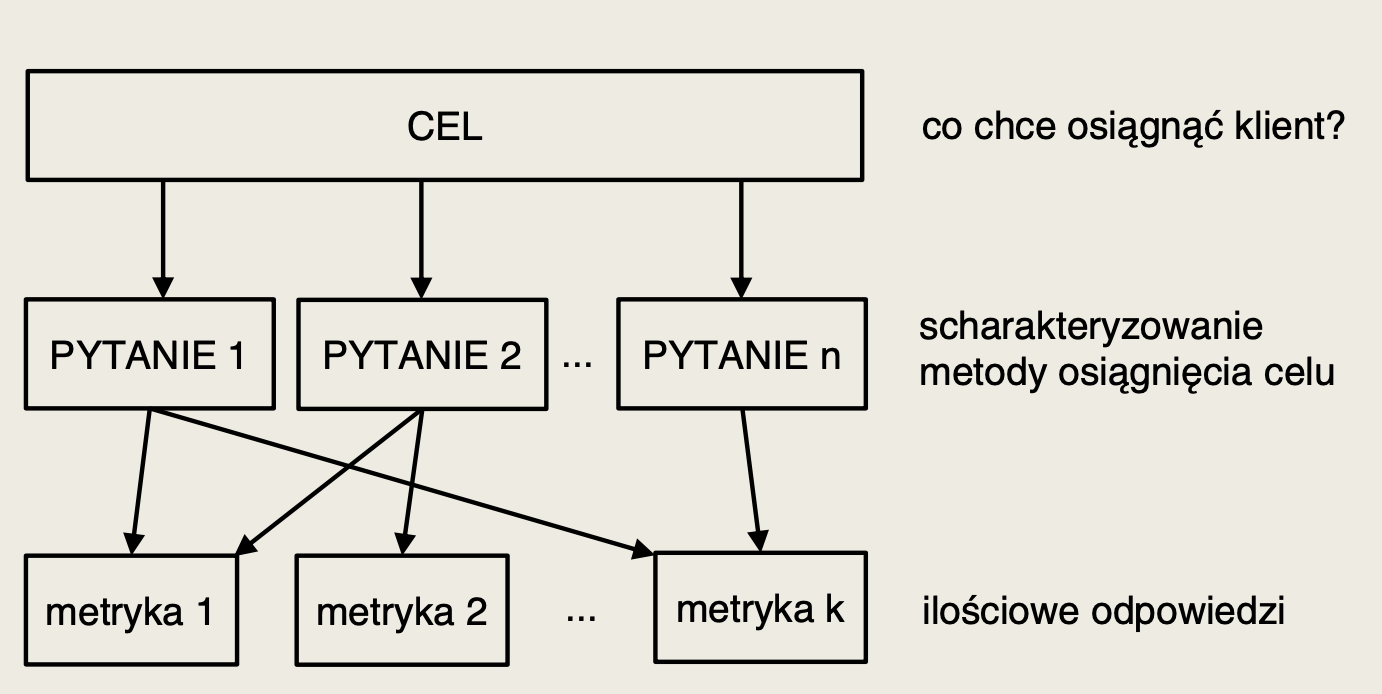
\includegraphics[width=\linewidth]{gqm.png}
    \end{figure}

    \begin{table}[H]
        \begin{center}
            \begin{tabular}{p{8cm} p{8cm}}
                \multicolumn{2}{c}{\textbf{Miary wolumenowe kodu}} \\

                \begin{itemize}
                    \item \textbf{LOC (Lines of Code)}
                    \begin{itemize}
                        \item prosta, niezawodna, wspierana narzędziami metoda
                        \item problem: dokładny pomiar dopiero po implementacji – problem: nie mierzy tego, co program robi
                    \end{itemize}
                \end{itemize}
                &
                \begin{itemize}
                    \item \textbf{FP (Function Points)}
                    \begin{itemize}
                        \item mierzy tzw. punkty funkcyjne
                        \item zaleta: można mierzyć na etapie projektu
                        \item zaleta: pomiar niezależny od języka programowania – wada: bardziej skomplikowana metoda liczenia
                    \end{itemize}
                \end{itemize}
            \end{tabular}
        \end{center}
    \end{table}

    \begin{table}[H]
        \begin{center}
            \begin{tabular}{p{8cm} p{8cm}}
                \multicolumn{2}{c}{  \textbf{Metryki złożoności strukturalnej}} \\
                \begin{itemize}
                    \item \textbf{rozmiar} (LOC, FP)
                    \item \textbf{złożoność cyklomatyczna} (stopień komplikacji kodu) [zalecane $<$ 10]
                    \item \textbf{złożoność Halsteada} (\# operatorów i operandów); krytykowana!
                    \item \textbf{przepływ informacji} (z i do modułu)
                    \item \textbf{złożoność systemu} (dla pomiaru pielęgnowalności)
                \end{itemize}
                &
                \begin{itemize}
                    \item metryki \textbf{strukturalne dla OOP}
                    \begin{itemize}
                        \item \textbf{WMC} (Weighted Methods defined per Class) [zalecane $<$ 100]
                        \item \textbf{DIT} (Depth of Inheritance Tree) [zalecane jak najmniejsze]
                        \item \textbf{NOC} (Number Of Children) [zalecane $<$ 40]
                        \item \textbf{CBO} (Coupling Between Objects) [zalecane $<$ 6]
                        \item \textbf{RFC} (Response For a Class) [zalecane $<$ 100, $<$ 5*liczba metod]
                        \item \textbf{LCOM} (Lack Of Cohesion) [zalecane jak najmniejsze]
                    \end{itemize}
                \end{itemize} \\
            \end{tabular}
        \end{center}
    \end{table}

    \textbf{Metryki złożoności konceptualnej} dotyczą trudności w zrozumieniu wymagań/kodu/itp.\\

    \textbf{Metryki złożoności obliczeniowej} dotyczą złożoności obliczeń programu w trakcie jego wykonania.

    \begin{table}[H]
        \begin{center}
            \begin{tabular}{p{8cm} p{8cm}}
                \multicolumn{2}{c}{\textbf{ Najczęstsze metryki defektów}} \\
                \begin{itemize}
                    \item liczba defektów
                    \item gęstość defektów = liczba defektów / objętość kodu
                    \item częstość defektów = liczba defektów / jednostkę czasu
                \end{itemize}
                &
                \begin{itemize}
                    \item odsetek wykrytych defektów = wykryte defekty / wszystkie defekty
                    \item wzorzec powstawania defektów
                \end{itemize} \\
            \end{tabular}
        \end{center}
    \end{table}

    \begin{table}[H]
        \begin{center}
            \begin{tabular}{p{8cm} p{8cm}}
                \multicolumn{2}{c}{\textbf{Modele statyczne defektów}} \\
                \begin{itemize}
                    \item Model fazowy.
                    \item Modele zmian w kodzie.
                \end{itemize}
                &
                \begin{itemize}
                    \item Model Rayleigha - opisuje rozkład znajdowania defektów w czasie.
                \end{itemize}
            \end{tabular}
        \end{center}
    \end{table}

    \textbf{Posiew defektów} (fault seeding) – metoda sztucznego wprowadzania defektów do kodu w
    celu sprawdzenia efektywności istniejących testów; np \textbf{testowanie mutacyjne}.

    \textbf{Wstrzykiwanie defektów} (fault injection) – metoda sztucznego wprowadzania defektów/wywoływania
    awarii, w celu sprawdzenia jak program radzi sobie z nietypowymi, błędnymi, „dziwnymi” sytuacjami.

    \textbf{Analiza mutacyjna} – wykorzystanie testowania mutacyjnego jako modelu predykcyjnego defektów.

\end{document}